%%%%%%%%%%%%%%%%%%%%%%%%%%%%%%%%%%%%%%%%%%%%%%%%%%%%%%%%%%%%%%%%%%%%%%%%%%%%%%%
% intro.tex: Introduction to the thesis
%%%%%%%%%%%%%%%%%%%%%%%%%%%%%%%%%%%%%%%%%%%%%%%%%%%%%%%%%%%%%%%%%%%%%%%%%%%%%%%%
\chapter{Introduction}
\label{intro_chapter}
%%%%%%%%%%%%%%%%%%%%%%%%%%%%%%%%%%%%%%%%%%%%%%%%%%%%%%%%%%%%%%%%%%%%%%%%%%%%%%%%

The Standard Theory of particle physics (ST) \cite{weinbergSM,salamSM} 
is a quantum field theory that describes the fundamental components of matter and their interactions; 
it predicts the existence of particles shown in Figure \ref{fig:structureOfSM}.  Over the past several 
decades particle colliders have tested the ST, and many of its predictions have been substantiated by 
experimental evidence.

\begin{figure}[h]
	\centering
	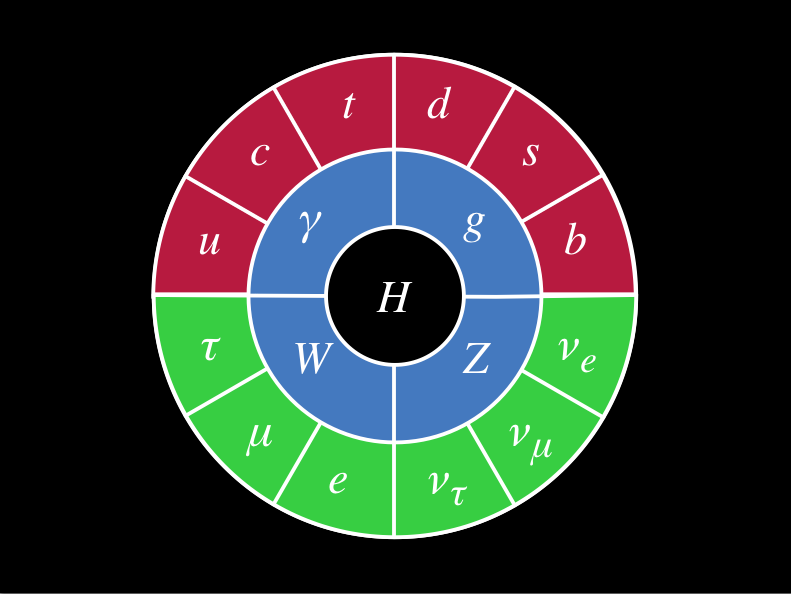
\includegraphics[width=1.0\textwidth]{figures/SM_particles_circularRep.png}
	\caption{Particles predicted by the Standard Model \cite{smParticles}.}
	\label{fig:structureOfSM}
\end{figure}

Neutrinos and the weak interaction played an important role in the development of the SM.  
Neutrinos were first proposed in 1929 to preserve energy conservation in beta decays, and were first 
substantiated by experimental evidence \cite{firstNuDiscovery} of the electron neutrino in 1956.  
Subsequent predictions of muon and tau neutrinos were later substantiated 
by experimental evidence \cite{muNuDiscovery,tauNuDiscovery}.  Neutrinos were predicted to interact only through weak 
interactions, so advances in the understanding of neutrino physics and the theory of weak interactions often coincided.  
A 1932 theoretical model of the weak interaction was proposed to explain beta decay, and included a massless 
neutral lepton later identified as the electron neutrino.  In the 1950s experimental measurements of 
hadron decay rates through the weak interaction, like $K^{+} \rightarrow 2\pi, 3\pi$, motivated new 
models of the weak interaction that did not conserve parity.  Parity violation in weak interactions was 
substantiated by experimental evidence \cite{weakParityViolation} in 1957.  Developed in the following decade, the 
SM predicted the existence of three massless neutrinos\footnote{At the time only two were supported 
by experimental evidence}, and predicted the weak interaction could be modeled as a parity violating 
quantum field theory.

The success of the SM is exemplified by the quantum field model of electromagnetic and weak (electroweak) 
interactions.  The electroweak model predicts the existence of a massive, neutral gauge boson, the $Z$, 
that mediates weak interactions between fermions.  Existence of the $Z$ was first substantiated by 
observations of neutral current scattering between neutrinos \cite{nuScattering} in 1973.  Later at 
LEP and the Tevatron, precise measurements of electroweak coupling strengths and gauge boson ($\gamma$, $W$, $Z$) 
masses put indirect limits on the Higgs boson mass.  The Higgs boson was observed in 2012 at the Large Hadron Collider 
(LHC) by the ATLAS and CMS experiments, and its mass\cite{combinedHiggsResult} of 125 $\GeV$ was consistent 
with previous electroweak limits.

The SM predicts many experimental observations of the universe, but there are indications that the SM is 
not a complete model of the universe.  Within the electroweak sector discussed previously, the SM does 
not predict the experimentally observed baryon-antibaryon asymmetry or neutrino oscillaions.  Neutrino flavor 
oscillations were first predicted in 1957, and are supported by experimental evidence 
\cite{kamiokandeTwo,solarNuSummary,NOvAresults,mainzPhaseIIResults,t2kResults}.  This evidence substantiates 
models with massive fermionic neutrinos, and conflicts with the SM.  The SM predicts the universe has more 
baryons than antibaryons due to CP violation in the electroweak model, but the experimentally observed 
asymmetry is larger than predicted \cite{surveyOfExtensions}.  Left-Right Symmetric (LRS) extensions of 
the SM predict massive neutrinos and a baryon-antibaryon asymmetry consistent with experimental observations, 
and retain SM predictions supported by experimental evidence.

LRS models extend the SM electroweak model by adding a $SU(2)_{R}$ gauge group and three heavy, right-handed 
neutrinos \nul.  Due to the new gauge group, LRS models predict a new charged weak boson \WR that couples to 
\nul and all right-handed SM fermions.  The \WR coupling to SM quarks enables a search for LRS models using 
data collected from proton-proton collisions at the CERN LHC.  In this thesis, a search for heavy neutrinos \nul 
and a \WR boson in events with two charged leptons and two jets collected by the CMS experiment in 2015 
is presented.

%%%%%%%%%%%%%%%%%%%%%%%%%%%%%%%%%%%%%%%%%%%%%%%%%%%%%%%%%%%%%%%%%%%%%%%%%%%%%%%%
